%!TEX root = ../thesis.tex

\thispagestyle{myheadings}

\graphicspath{{Body/Figures/ExperimentalOverview/Decay/}{Body/Figures/TrackingFigures/TrackerPics/}{Body/Figures/ExperimentalOverview/Ring/}{Body/Figures/ExperimentalOverview/Auxiliary/}}

\chapter{Principle Technique of E989}
\label{chapter:E989}

As referenced in \equref{eq:torque}, a particle in a magnetic field will experience a torque which attempts to line up the magnetic dipole moment of the particle with the external field. Because of this, in a dipole field a particles spin will turn at the Larmour precesssion frequency \cite{Jackson}
        \begin{align} \label{eq:ws}
            \vec{\omega}_{s} = -g\frac{q}{2m}\vec{B} - (1-\gamma)\frac{q}{\gamma m}\vec{B},
        \end{align}
where as before $m$ is the particles mass, $q = \pm e$ where $e$ is the elementary charge, \g is the g-factor, $\gamma$ is the Lorentz relativistic factor, and $B$ is an external magnetic field. The second term is a relativistic correction to the precession frequency called Thomas precession \cite{Jackson}. Similarly, a particle with some momentum will orbit at the cyclotron frequency
        \begin{align} \label{eq:wc}
            \vec{\omega}_{c} = -\frac{q}{\gamma m}\vec{B}.
        \end{align}
By taking the difference between these two frequencies we arrive at the "spin difference frequency"
        \begin{align} \label{eq:wasimple}
            \vec{\omega}_{a} = \vec{\omega}_{s} - \vec{\omega}_{c} = -\frac{g-2}{2}\frac{q}{m}\vec{B} = - a \frac{q}{m}\vec{B},
        \end{align}
a frequency that is directly proportional to the anomalous magnetic moment $a$. Briefly note that if $g = 2$ as in a Dirac theory, then the particles spin would turn at the same rate as the momentum vector, and this spin difference frequency \wa would be identically 0. If this spin difference frequency for a muon and the external magnetic dipole field can be measured, then the anomalous magnetic moment of the muon \amu can be measured. Introductory descriptions for both will be given here, while the details are left to \chapref{chapter:SpinPrecessionMeasurement} and 
\chapref{chapter:MagneticFieldMeasurement} respectively.


\section{Measuring \texorpdfstring{\wa}{wa}}
\label{section:WaIntro}

How can \wa for muons be measured? The answer lies with two key points in the dynamics of muon decay. Positive muons decay to a positron and two neutrinos, as shown in \figref{fig:mudecay}. The first point is that because of the parity violating nature of the weak interaction, the decay positron will be preferentially emitted right-handed, with its spin directed in the same direction as its momentum \cite{Bucksbaum}. The second key point is that angular momentum must be conserved. Consider the most extreme examples of maximum and minimum energy positrons as shown in \figref{fig:MuonDecayImproved}. In the muon rest frame, decay positrons with maximum energy will be emitted opposite to the two neutrinos. Since neutrinos and anti-neutrinos must be left and right-handed respectively, thus having their spins anti-parallel and parallel to their momentum, by the law of conservation of angular momentum the positron must have its spin be parallel to the spin of the muon at the time of the decay. By the opposite argument, decay positrons emitted with minimum energy such that the neutrinos are ejected opposite to one another must have their spins be anti-parallel to that of the muon at the time of decay. These two points combined together means that higher energy decay postrons will preferentially be emitted in directions parallel to the muon spin at the time of decay, while lower energy decay positrons will preferentially be emitted in directions anti-parallel to the muon spin at the time of the decay. 

\begin{figure}[]
\centering
    \subcaptionbox{$\mu^{+}$ decay through a $W^{+}$ boson to a positron, muon anti-neutrino, and an electron neutrino. This is the dominant decay mode.
    \label{fig:mudecay}}
    {
    \centering
        \begin{tikzpicture}[baseline=(o.base)]
        \begin{feynhand}
        \large
        \setlength{\feynhandlinesize}{1pt}
        \vertex [dot] (o) at (0,0);
        \vertex (a) at (-2,0) {$\mu^{+}$}; 
        \vertex (b) at (1.5,1.5) {$\overline \nu_{\mu}$}; 
        \vertex (c) at (1.5,-1.5);
        \vertex (d) at (3,0) {$\nu_{e}$};
        \vertex (e) at (3,-3) {$e^{+}$};
        \propag [anti fermion] (a) to (o);
        \propag [fermion] (b) to (o);
        \propag [boson] (o) to [edge label' = $W^{+}$] (c);
        \propag [fermion] (c) to (d);
        \propag [anti fermion] (c) to (e);
        \end{feynhand}
        \end{tikzpicture} 
    }
    \hspace{10mm}
    \subcaptionbox{$\pi^{+}$ decay through a $W^{+}$ boson to a $\mu^{+}$.
    \label{fig:pidecay}}
    {
    \centering
        \begin{tikzpicture}[baseline=(o.base)]
        \begin{feynhand}
        \large
        \setlength{\feynhandlinesize}{1pt}
        \vertex [dot] (o) at (0,0);
        \vertex (a) at (-1.5,1.5) {$u$}; 
        \vertex (b) at (-1.5,-1.5) {$\overline d$}; 
        \vertex (c) at (2,0);
        \vertex (d) at (3.5,1.5) {$\mu^{+}$};
        \vertex (e) at (3.5,-1.5) {$\nu_{\mu}$};
        \propag [fermion] (a) to (o);
        \propag [anti fermion] (b) to (o);
        \propag [boson] (o) to [edge label = $W^{+}$] (c);
        \propag [anti fermion] (c) to (d);
        \propag [fermion] (c) to (e);
        \end{feynhand}
        \end{tikzpicture}  
    }
\caption[Feynman diagrams for muon and pion decay]{Feynman diagrams for muon (left) and pion (right) decay.}    
\label{fig:DecayDiagrams}
\end{figure}

\begin{figure}[]
    \centering
    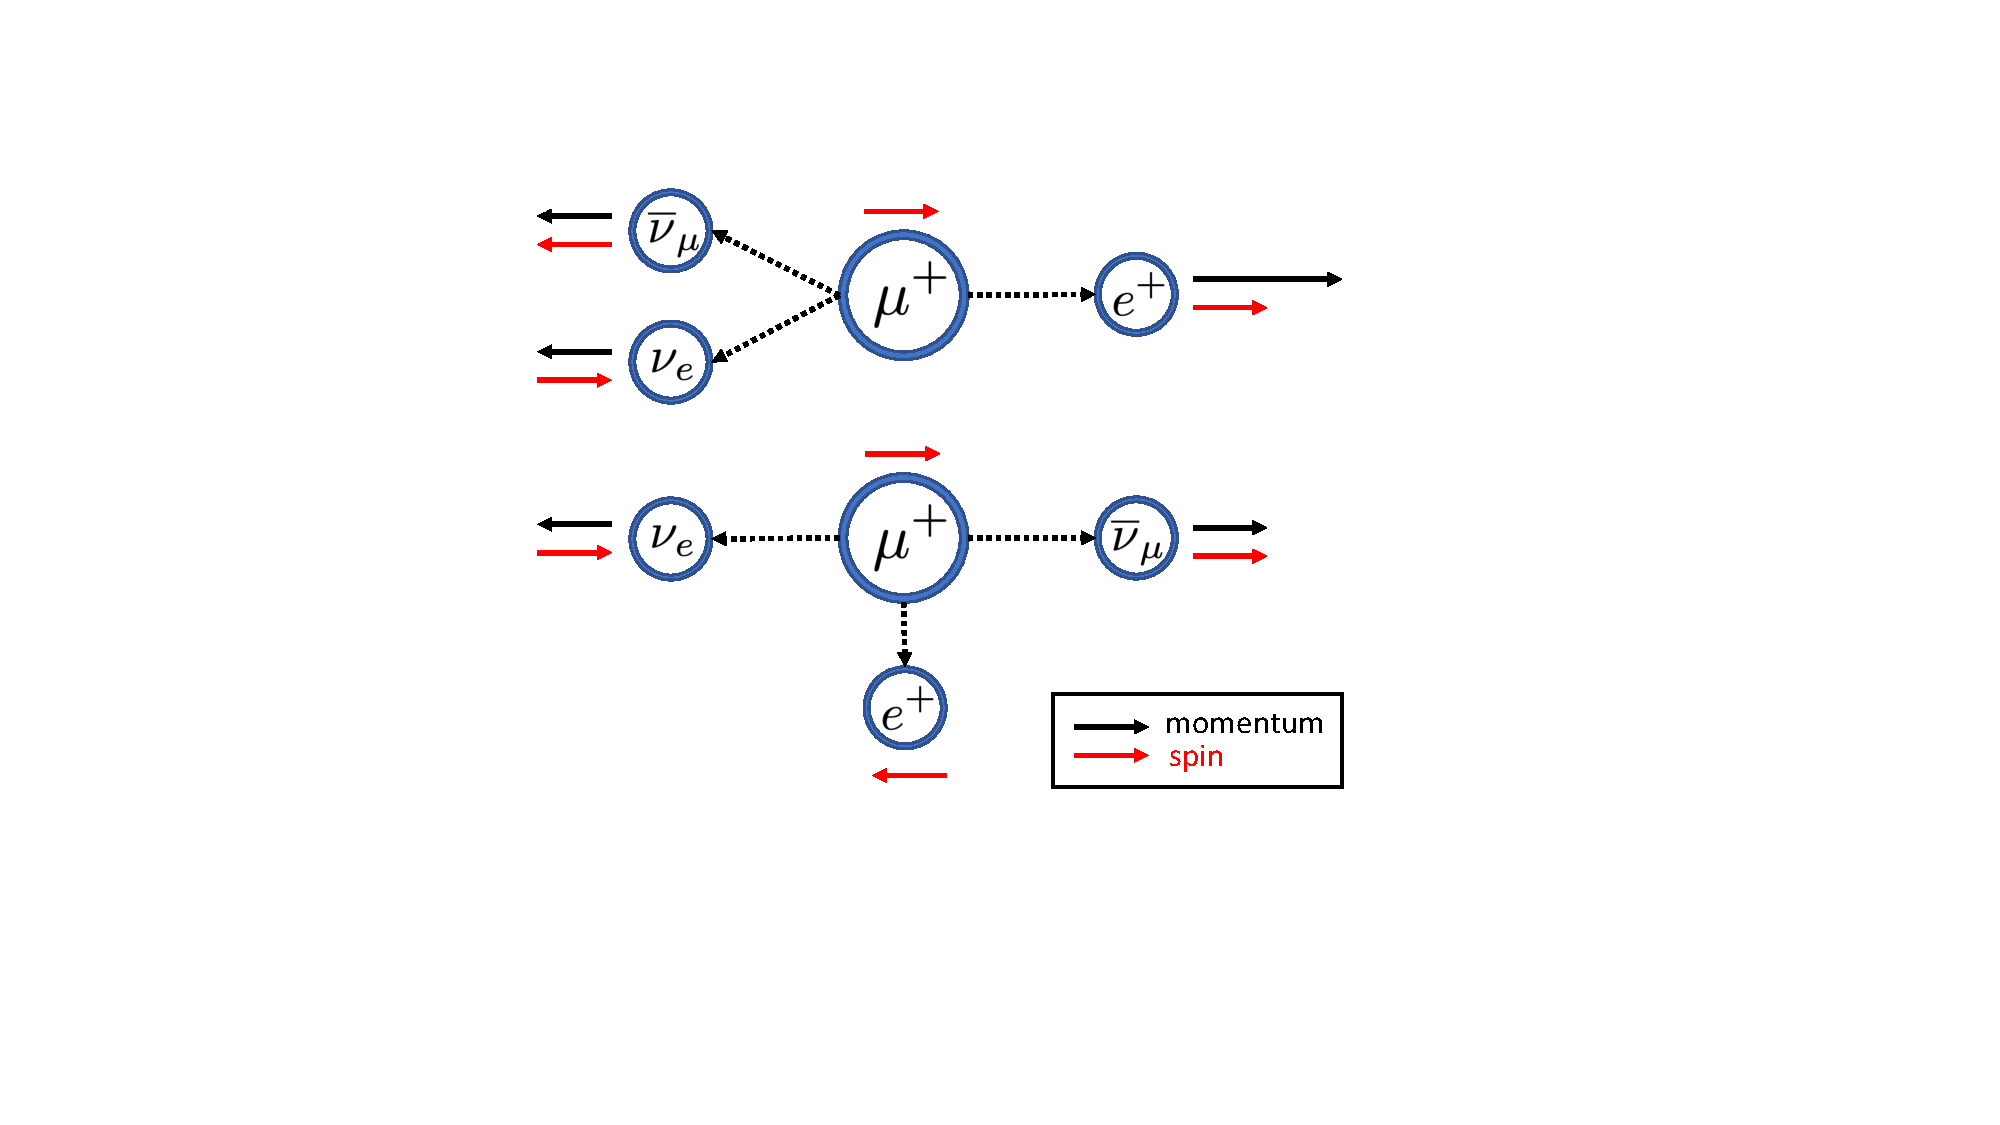
\includegraphics[width=0.6\textwidth]{MuonDecayImproved}
    \caption[Muon decay pictures for maximum and minimum energy decay positrons]{Muon decay pictures for maximum and minimum energy decay positrons. Due to the conservation of angular momentum and the single possible helicity states of the decay neutrinos, the spin of the decay positron is exactly parallel to the spin of the muon at the time of the decay for maximum energy decay positrons (top), or anti-parallel for minimum energy decay positrons (bottom).}
    \label{fig:MuonDecayImproved}
\end{figure}


This correlation between the emitted direction of the decay positron and the spin of the muon is the signature needed to measure \wa. By placing an ensemble of polarized muons within a magnetic storage ring, those muons will orbit at the cyclotron frequency and their spins will precess at the Larmour frequency. As they go around the ring they will decay to positrons whose energy and decay directions contain information about the spin of the muon. The differential decay distribution in the muon rest frame is described by \cite{Bucksbaum}
        \begin{align} \label{eq:diffdecaydist}
            dP(y, \theta) \propto N(y)[1 \pm A(y)\cos(\theta)]dy d\Omega,
        \end{align}
where $y=E/E_{max}$ is the energy fraction of the positron, $N(y)$ is the number distribution of decay positrons, $A(y)$ is the so called asymmetry encoding the preferred direction, $\theta$ is the angle between the spin of the muon and the momentum of the positron $\cos^{-1}(\hat{p} \cdot  \hat{s})$, and the $\pm$ stands for the positive and negative muon respectively. Here the energy of the positron is assumed to be much greater than its mass. The number distribution and asymmetry are given by \cite{Bucksbaum}
        \begin{equation}
        \begin{aligned}
            N(y) &= 2y^{2}(3-2y^{2}), \\
            A(y) &= \frac{2y-1}{3-2y}, 
        \end{aligned}
        \end{equation}
and are shown in \figref{fig:NA2mrf}.




\begin{figure}[]
\centering
    \begin{subfigure}[]{0.45\textwidth}
        \centering
        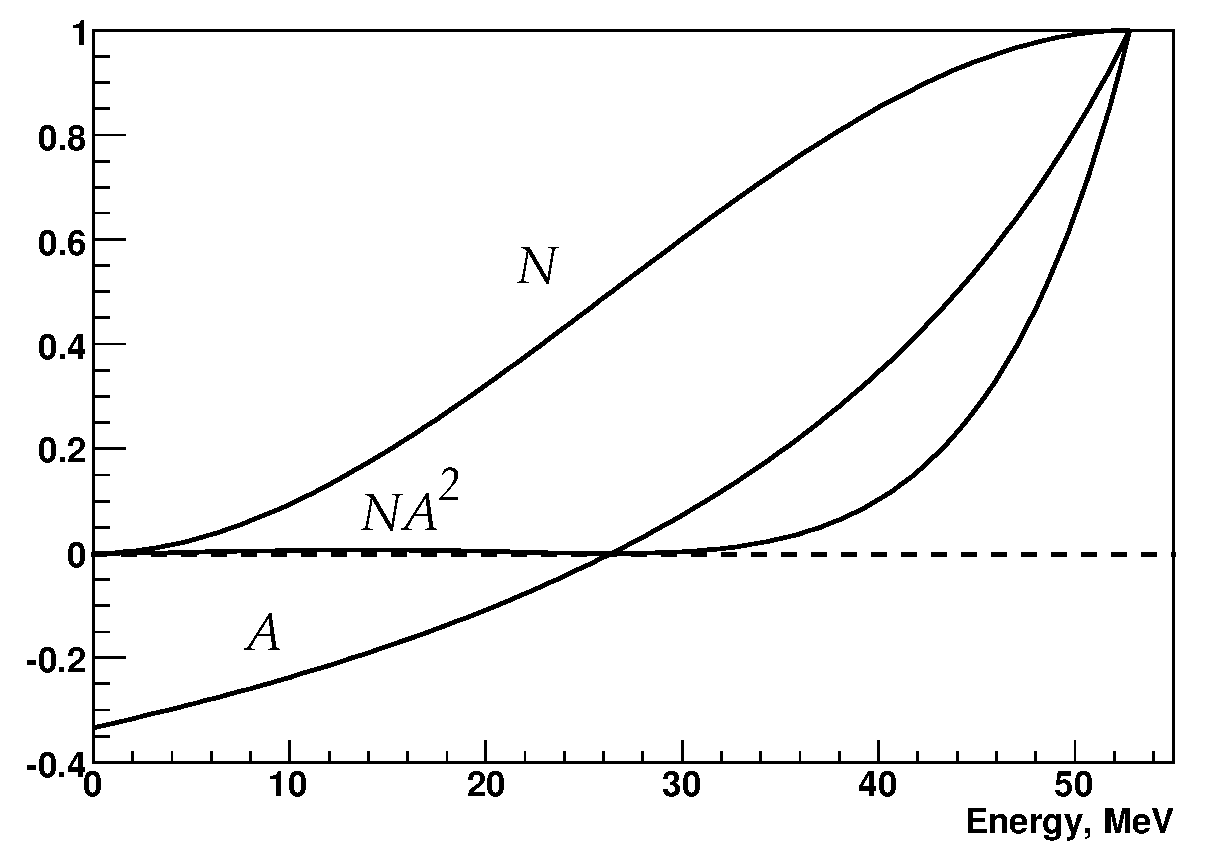
\includegraphics[width=\textwidth]{NA_mrf}
        \caption{Muon rest frame}
    \label{fig:NA2mrf}
    \end{subfigure}%
    \hspace{1cm}
    \begin{subfigure}[]{0.45\textwidth}
        \centering
        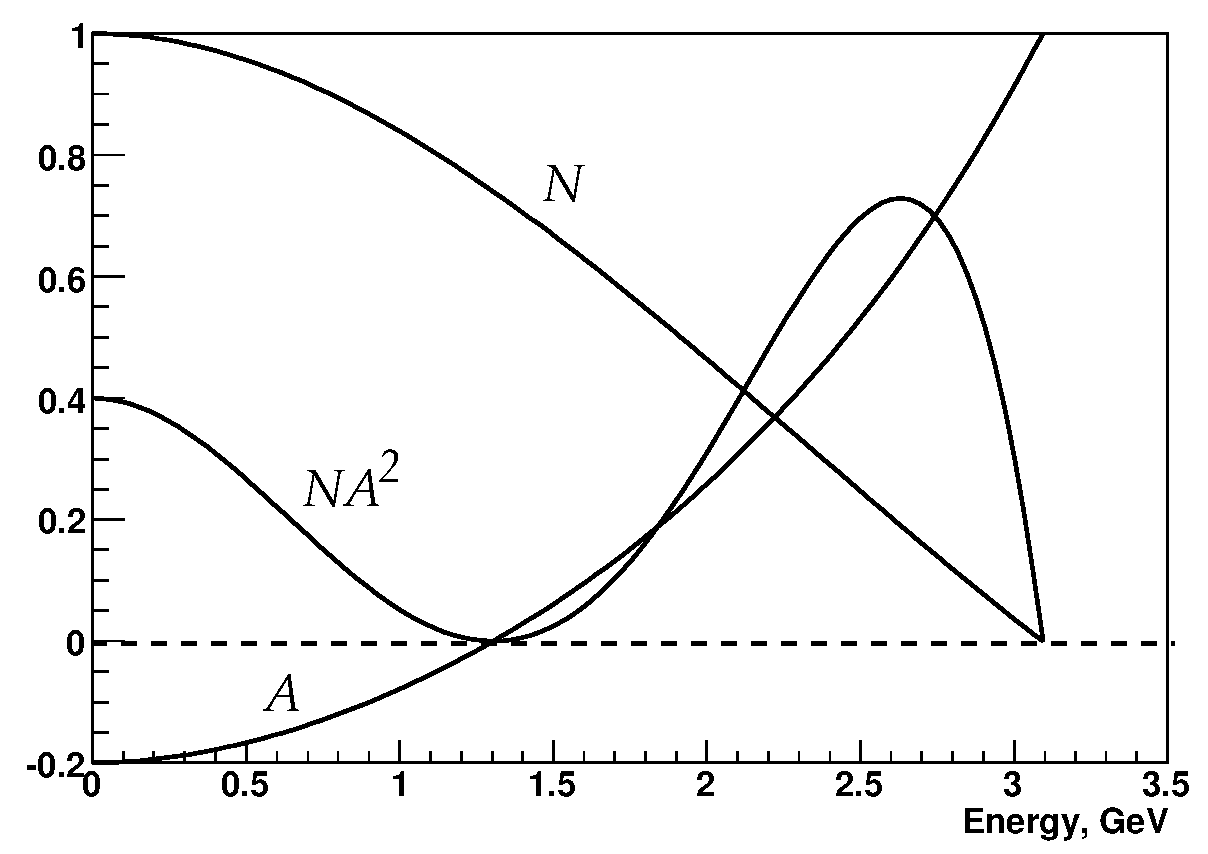
\includegraphics[width=\textwidth]{NA_lab}
        \caption{Lab frame}
    \label{fig:NA2lab}    
    \end{subfigure}
\caption[Number distribution and asymmetry for muon decay in the muon rest frame and lab frame]{Decay number distribution $N$ and asymmetry $A$ in the muon rest frame (left) and in the lab frame (right) as a function of positron energy with a maximum positron energy of 3.1 \GeV.}
\label{fig:NA2}
\end{figure}




Specifically, the number of positrons emitted in the forward direction above some energy threshold will be modulated by \wa


Specifically, the positrons emitted in the forward direction will be modulated by \wa as the muon spins precess about the momentum vector  


% positrons in the forward direction will be modulated by ... 

% By placing detectors in a subset of the decay region, 

% The number of high energy positrons seen in the calorimeters and trackers is modulated by the spin difference frequency

% In the laboratory frame there will thus be a correlation between the momentum of the decay positron and the muon spin

% To the equations for N and A...

% By measuring blah for an ensemble of .. 












\clearpage



In the presence of an electric field, which is useful in storing the muon beam within a dipole magnetic field, this expands to 
        \begin{align} \label{eq:waelectric}
            \vec{\omega}_{a} = -\frac{Qe}{m} [a_{\mu}\vec{B} - (a_{\mu} - \frac{1}{\gamma^{2}-1})(\vec{\beta} \times \vec{E}) ],
        \end{align}
where now the measurable quanties are vector quantities. Finally, for realistic cases of muon momentum which is non-orthogonal to the magnetic field, the spin difference frequency becomes
        \begin{align} \label{eq:wafinal}
            \vec{\omega}_{a} = -\frac{Qe}{m} [a_{\mu}\vec{B} - a_{\mu} (\frac{\gamma}{\gamma+1})(\vec{\beta} \cdot \vec{B})\vec{B} - (a_{\mu} - \frac{1}{\gamma^{2}-1})(\vec{\beta} \times \vec{E}) ].
        \end{align}
If the motion of the muons is largely perpendicular to the magnetic field, then the second term is small and can be corrected for. If the particles have a momentum of approximately 3.09 \GeV/c, the so called ``magic momentum,'' then the third term is small and can be corrected for. These will be talked about later.

In order to measure the spin difference frequency of the muon, a clever technique is used. Decay muons in the pion rest frame are 100\% polarized due to conservation of angular momentum and the fact that the decay neutrino must have a specific helicity. Within a pion beam then the highest and lowest energy decay muons are polarized. Muons will decay to positrons with a lifetime of about 2.2 $\mu$s, and the positrons with the highest energies will be correlated with the muon spin, a so called ``self-analyzing'' decay. The single available decay state for a maximum energy positron illustrates this in \figref{fig:MuonDecay}. Thus, by aquiring a large sample of polarized muons and injecting them into a storage ring 








-explain the physics
-explain how we get at the physics with our ring and detectors
-parity violation
-actually write out the decay states before explaining some things - well shouldn't these have been talked about before?? maybe not
-decay probabilities and all that
-don't measure all decay positrons
-By injecting a large ensemble of muons and 
-by measuring a subset of ensemble of muons....
-Careful with spin vs polarization





\begin{figure}[]
    \centering
    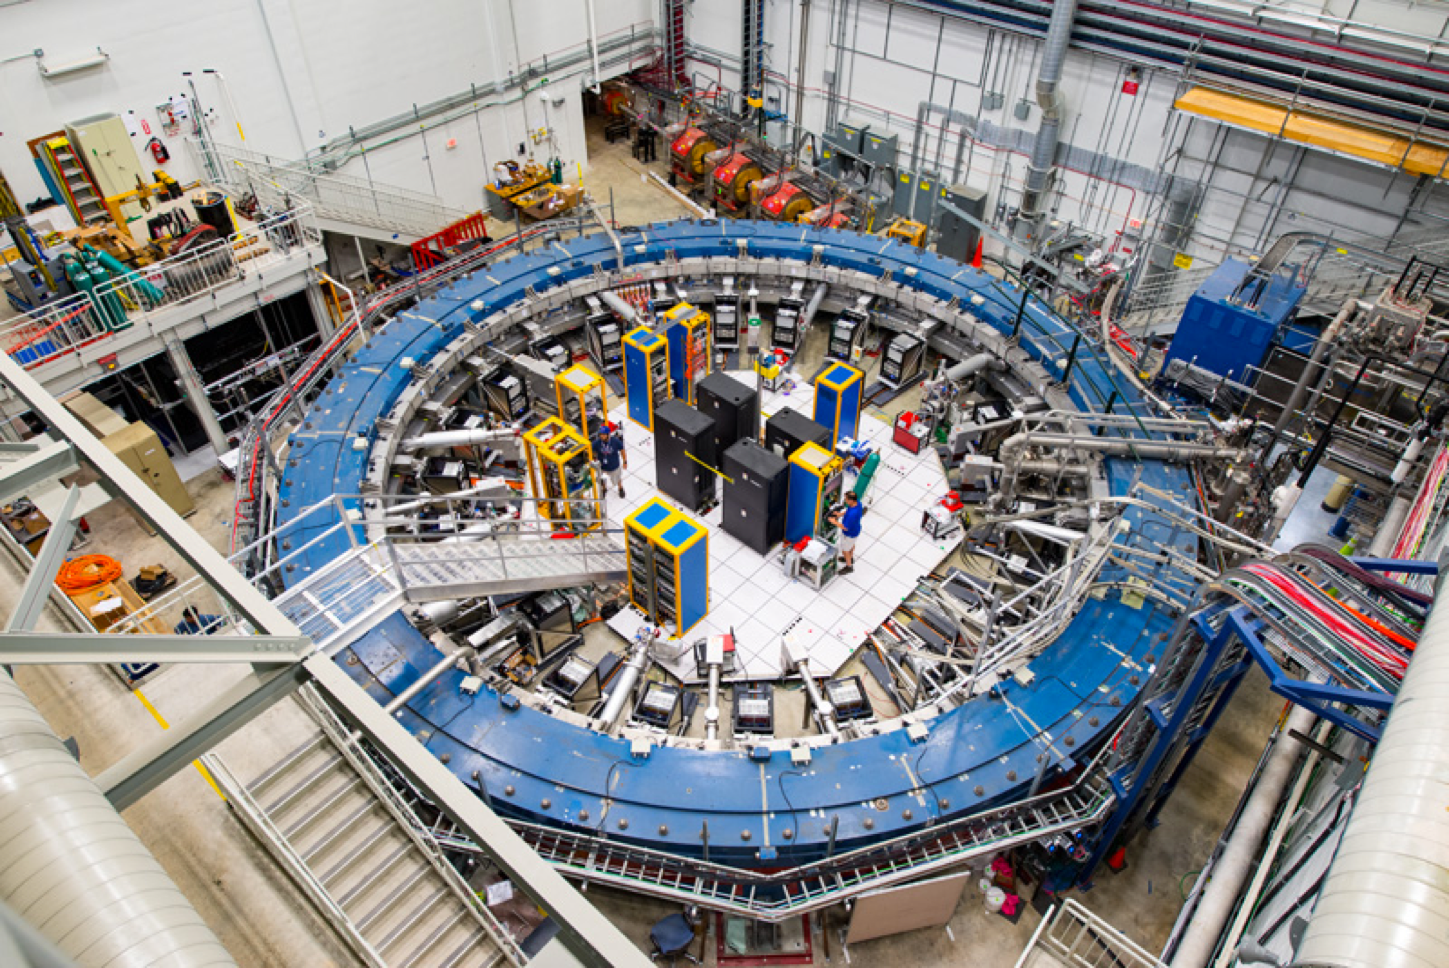
\includegraphics[width=0.9\textwidth]{ring}
    \caption[ring]{clean up and possibly replace}   
    \label{fig:ring}
\end{figure}





\section{Measuring B}
\label{sec:BIntro}






\section{Accelerator}
\label{sec:Accelerator}




\cite{Stratakis:2017uci}


\section{Injection}
\label{sec:Injection}

the inflector



\section{Storage}
\label{sec:Storage}

kickers and quads




